

\documentclass[14pt]{beamer}
\usepackage{pgf,tikz,pgfpages,amsmath,bm,fancyvrb,animate}
\usepackage{graphicx,bera,booktabs}
\usepackage[australian]{babel}
\usepackage[utf8]{inputenc}
\usepackage{url}

\usepackage{dsfont}

\usetheme{Monash}
\def\biz{\begin{itemize}[<+-| alert@+>]}
\def\eiz{\end{itemize}}
\def\ben{\begin{enumerate}[<+-| alert@+>]}
\def\een{\end{enumerate}}

\graphicspath{{../figures/}{../figures/book_figures/Chapter4/}{../figures/book_figures/Chapter3/}}

\title[5. Classification]{Business Analytics}
\author{Week 5\\ Classification}


\DefineShortVerb{\"}
\def\FancyVerbFormatCom{\color[rgb]{0.6,0,1}\relax}


\begin{document}

\begin{frame}[plain]{}
\maketitle
\begin{textblock}{11}(0.5,1.3){\color{white}\large
\textbf{ETC3250}}
\end{textblock}
\end{frame}


\begin{frame}{Outline}\fontsize{11}{14}\sf\tabcolsep=0.1cm
\centerline{\begin{tabular}{rlll}
\hline
\bf Week& \textbf{Topic} & \bf Chapter & \bf Lecturers\\
\hline
1  & Introduction to business analytics \& R     & 1    & Rob,Souhaib   \\
2  & Statistical learning                        & 2    & Rob,Souhaib\\
3  & Regression for prediction                   & 3    & Rob \\
4  & Resampling                                  & 5    & Rob, Souhaib \\
5  & Dimension reduction                         & 6,10 & Rob, Souhaib\\
6  & Visualization                               &      & Di \\
7  & Visualization                               &      & Di \\
8  & \textcolor{blue}{Classification}                              & 4  & Souhaib, Di\\
9  & Classification                              & 4,9  & Souhaib\\
-  & Semester Break \\
10 & Advanced classification                     & 8    & Di \\
11 & Advanced regression                         & 6    & Di \\
12 & Clustering                                  & 10   & Di
\end{tabular}}
\end{frame}

\begin{frame}{What is classification?}\large


\centerline{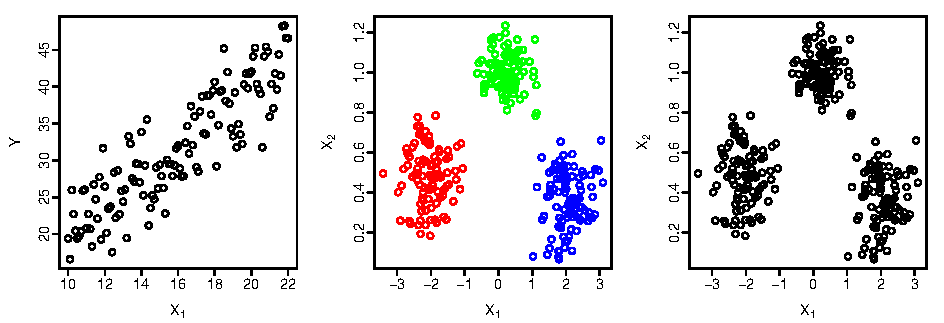
\includegraphics[width=12.2cm]{statlearn.pdf}}
\vspace{-1cm}
$$ \mathcal{D} = \{(x_i, y_i)\}_{i = 1}^N \text{~or~} \{x_i\}_{i = 1}^N, \quad x_i = (x_{i1}, \dots, x_{ip})^{T}$$


\begin{itemize}\normalsize
	\item Supervised learning: \textcolor{blue}{classification} and regression
	\item Unsupervised learning: clustering
\end{itemize}

\end{frame}

\begin{frame}{What is classification?}

The response variable $Y$ is \alert{qualitative}.
\begin{itemize}
\item e.g., email is one of ${\cal C} = (\text{spam},\text{ham})$
\item e.g., voters are one of ${\cal C} = (\text{Liberal},\text{Labor},\text{Green},\text{National},\text{Other})$
\end{itemize}
\structure{Our goals are:}
\begin{enumerate}
\item Build a classifier $C(x)$ that assigns a class label from ${\cal C}$ to a future unlabeled observation $x$.
\item Assess the uncertainty in each classification (i.e., the probability of misclassification).
\item Understand the roles of the different predictors among $X = (X_1,X_2,\dots,X_p)$.
\end{enumerate}
\end{frame}

\begin{frame}{Optimal classifier}

In place of MSE, we now use the \textcolor{blue}{error rate}:
\begin{block}{}
$$ E[I(Y \ne \hat{f}(X))] $$
\end{block} \pause
Suppose the $K$ classes in $\cal C$ are
numbered $1, 2, \dots, K$. Let
\begin{block}{}
\centerline{$
p_k(x) = \text{Pr}(Y = k\mid X = x),\qquad k = 1, 2, \dots , K.
$}
\end{block}
These are the \alert{conditional class probabilities} at $x$. \pause


Then the \alert{Bayes classifier} at $x$ is
\begin{block}{}
\centerline{$
C(x) = j\quad \text{if $p_j(x) = \max\{p_1(x), p_2(x), \dots, p_K(x)\}$}
$}
\end{block}

\end{frame}

\begin{frame}{Optimal classifier}
	
	
\begin{itemize}
\item The \alert{Bayes classifier} gives the minimum average test error rate, called the ``Bayes error rate'': $1-\text{E}\left(\max_j \text{Pr}(Y=j | X)\right)$

\item The ``Bayes error rate'' is the lowest possible error rate that could be achieved if we knew exactly the ``true'' probability distribution of the data.
\item It is analagous to the ``irreducible error'' in regression.
\item On test data, no classifier can get lower error rates than the Bayes error rate.
\item In reality, the Bayes classifier is not known.
\end{itemize}

\end{frame}


\begin{frame}{\normalsize Classification of classification methods}\large

%\url{https://en.wikipedia.org/wiki/Linear_classifier#Generative_models_vs._discriminative_models}

\begin{itemize}
	\item \alert{Generative} and \alert{discriminative}  models
	\begin{itemize}
	\item $P(X, Y)$ vs $P(Y|X)$
	\end{itemize}

	\item Logistic regression
	\begin{itemize}
	\item \textcolor{red}{Today}
	\end{itemize}

	\item Linear Discriminant Analysis
	\begin{itemize}
	\item \textcolor{blue}{Thursday}
	\end{itemize}
	
	\item Support Vector Machines
	\begin{itemize}
	\item \textcolor{blue}{Monday, next week}
	\end{itemize}
	
	\item k-Nearest Neighbours
	\begin{itemize}
	\item \textcolor{blue}{Thursday, next week}
	\end{itemize}
	
	\item Advanced methods: Boosting, Random Forests, etc
	\begin{itemize}
	\item \textcolor{blue}{Week 10}
	\end{itemize}
\end{itemize}

\end{frame}

\begin{frame}{\large Classification with linear regression}\large

\begin{itemize}
	\item How would you use linear regression for classification?
	\item Binary classification
	\begin{itemize}
	\item $Y = 0$ (stroke) and $Y = 1$ (drug overdose) \pause
	\item $E[Y | X] = P(Y = 1|X)$
	\item Problem: estimates outside $[0, 1]$ \pause
	\end{itemize}
	
	\item Multi-class classification
	\begin{itemize}
	\item $Y = 1$ (stroke), $Y = 2$ (drug overdose) and $Y = 3$ (epileptic seizure) \pause
	\item $Y = 1$ (epileptic seizure), $Y = 2$ (stroke) and $Y = 3$ (drug overdose) \pause
	\item Problem: Each coding will produce fundamentally different linear models
	\end{itemize}
	
\end{itemize}

\end{frame}

\begin{frame}{Why not linear regression?}

\vspace{-.5cm}
\centerline{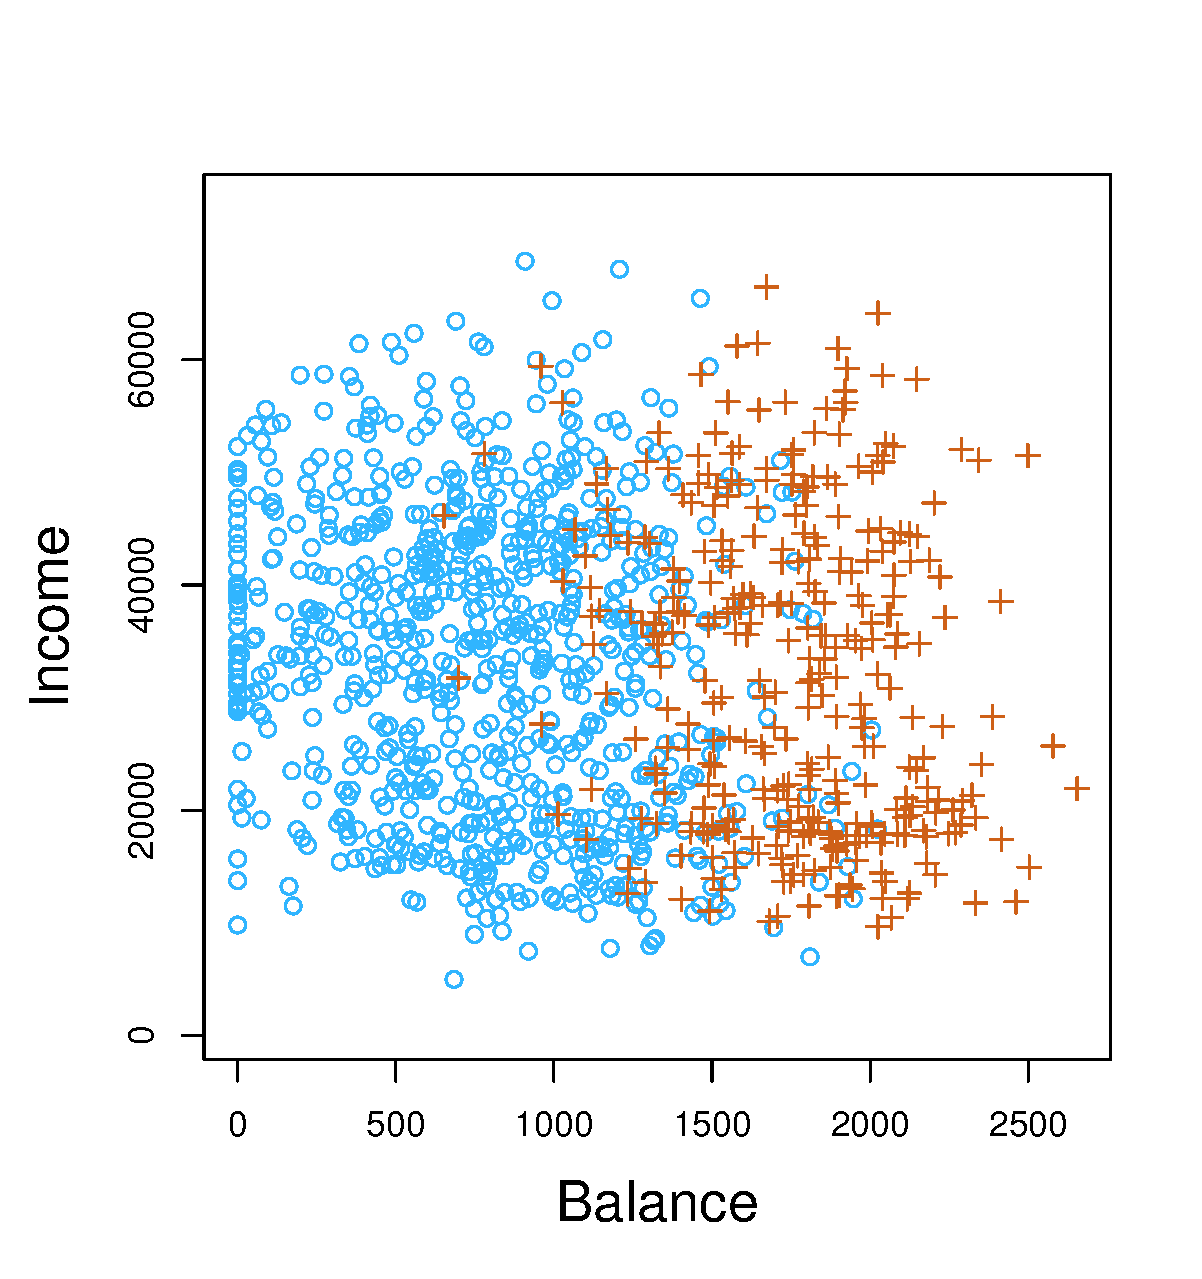
\includegraphics[width=.4\textwidth]{4-1a}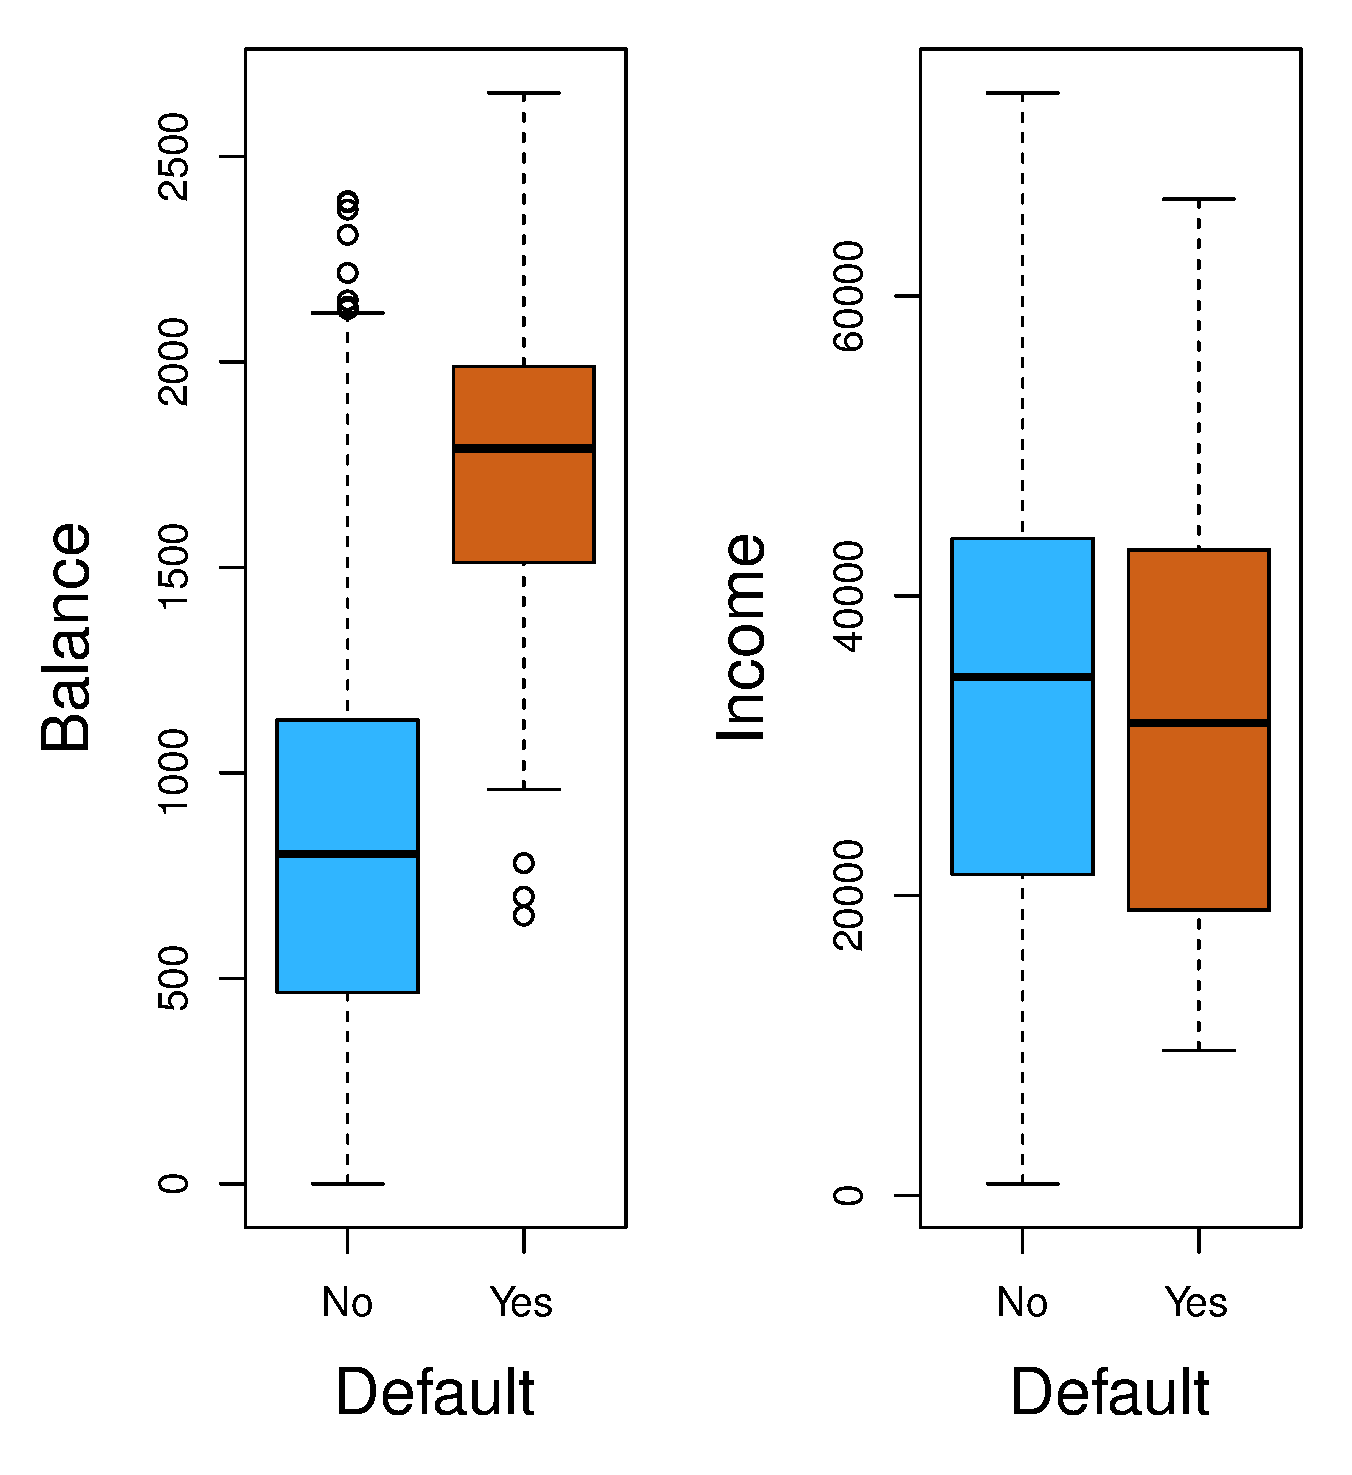
\includegraphics[width=.35\textwidth]{4-1b}}
\vspace{-.5cm}

\begin{minipage}{\linewidth}
\begin{minipage}{.42\linewidth}
\centerline{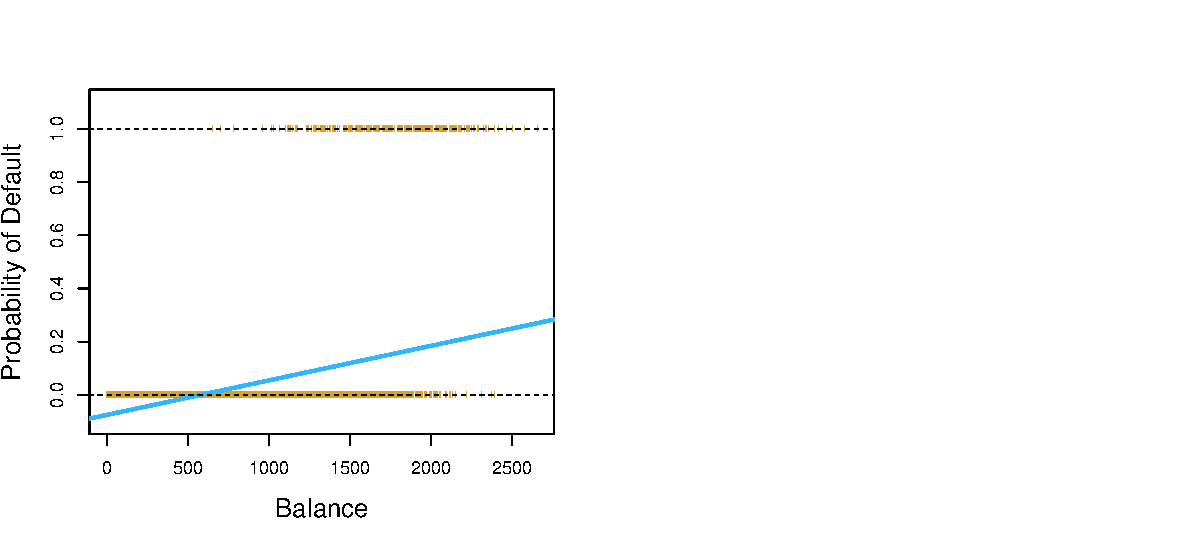
\includegraphics[width=.8\textwidth]{4-2a}}
\end{minipage}
%\hfill
\begin{minipage}{.56\linewidth} \small
$ p(X) = P(Y = 1|X) = \beta_0 + \beta_1 X$

$\scriptsize p(\text{\alert{balance}}) = p(\text{\alert{default} = \alert{Yes}}|\text{\alert{balance}})$

\vspace{.5cm}

$\text{\alert{default} = \alert{Yes}} \text{~if~} \scriptsize \hat p(\text{\alert{balance}}) > 0.5 $

Problem: $\hat p(X) > 0$ or $\hat p(X) <0$ 
\end{minipage}
\end{minipage}


\end{frame}

\begin{frame}{Logistic regression}\large
%\vspace{-1cm}

\centerline{$p(X) = \text{logistic}(\beta_0 + \beta_1 X) = \frac{e^{\beta_0 + \beta_1 X}}{1 + e^{\beta_0 + \beta_1 X}} $}

%\vspace{-1cm}
\centerline{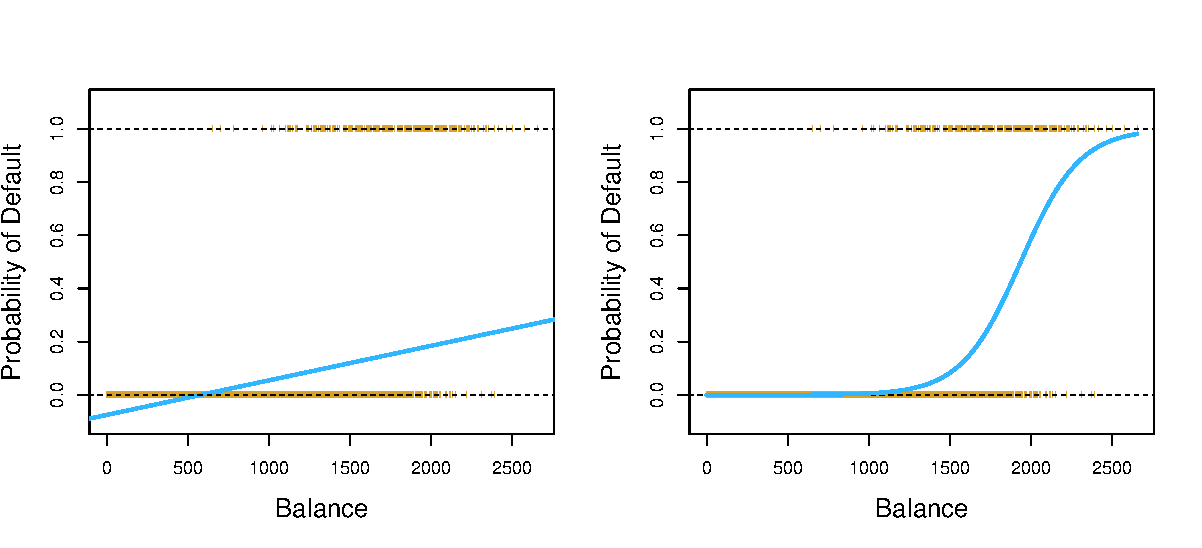
\includegraphics[width=\textwidth]{4-2}}

\centerline{$ l(\beta_0, \beta_1) = \prod_{i: y_i = 1} p(x_i) \prod_{i': y_{i'} = 0} (1 - p(x_{i'}))$}


\end{frame}
%$$p(X) = \text{logistic}(\beta_0 + \beta_1 X)$$ 
%where $\text{logistic}(x) = \frac{e^x}{1 + e^{x}}$
% $$p(X) = \text{logistic}(\beta_0 + \beta_1 X), \text{logistic}(x) = \frac{e^x}{1 + e^{x}}$$ 

\begin{frame}{Logistic regression}\large

\centerline{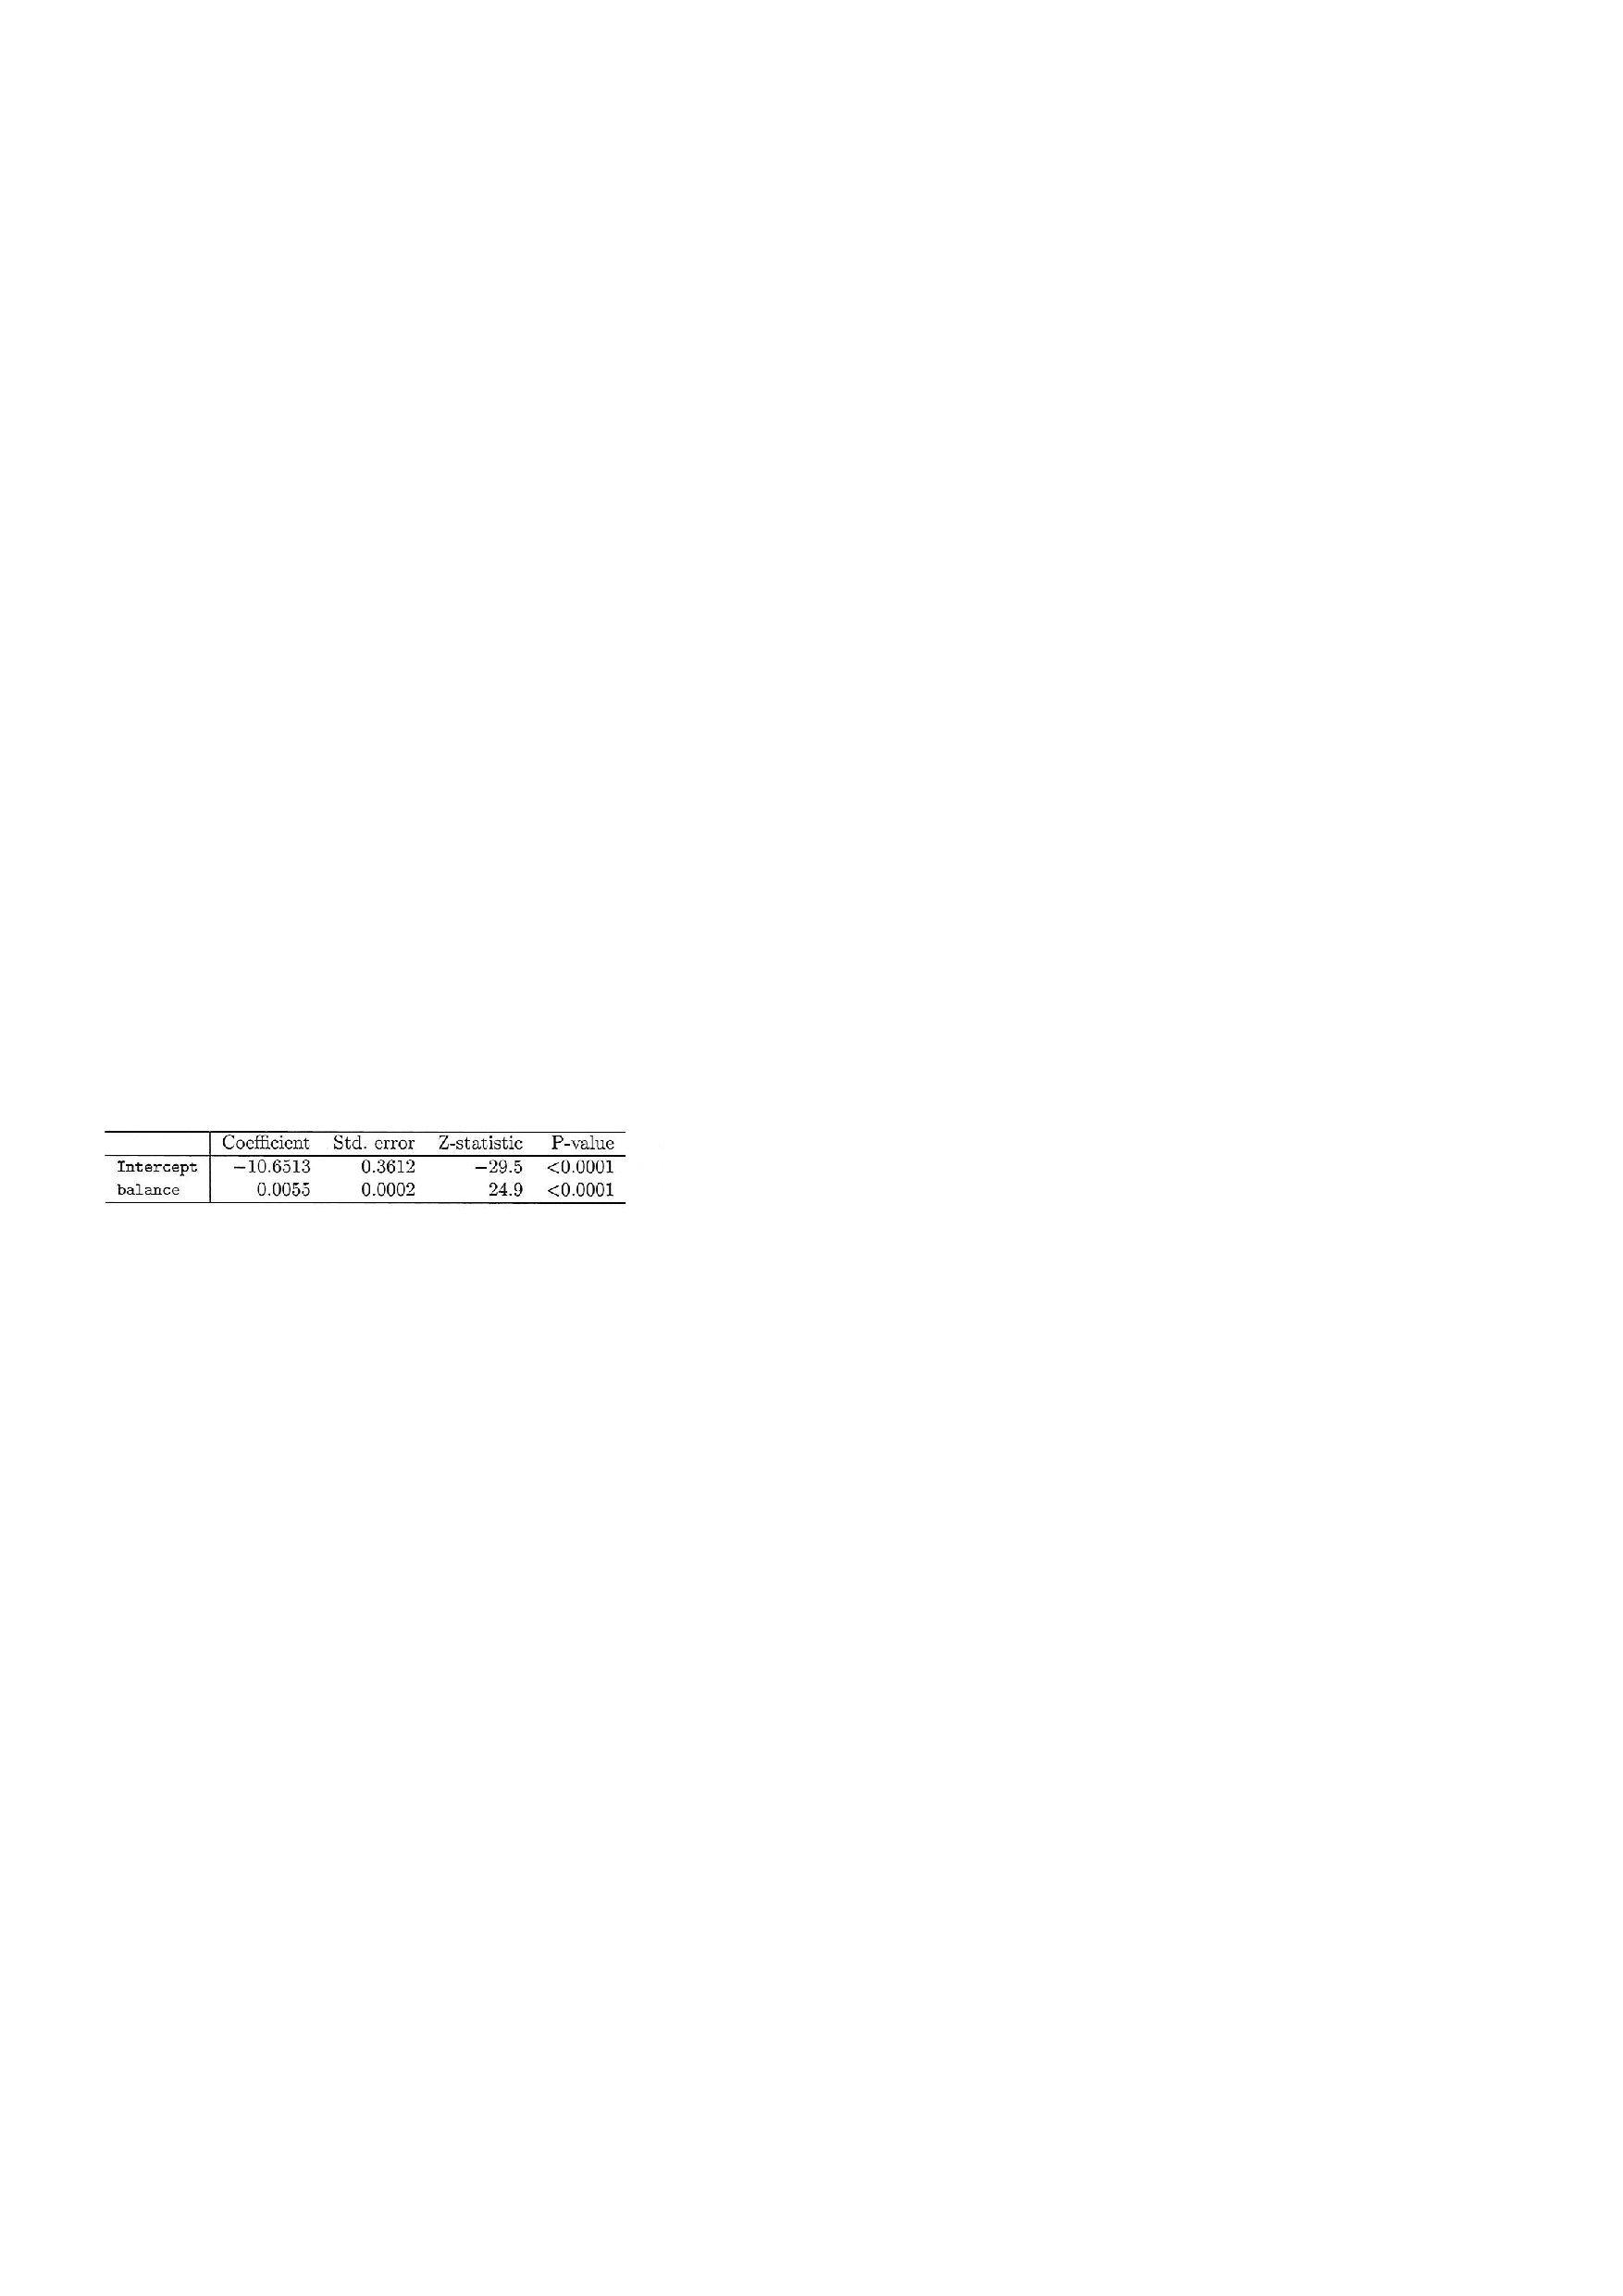
\includegraphics[width=.7\textwidth]{Table1}}

\centerline{
\includegraphics[width=.7\textwidth]{Table2}} 

TABLE 3.1

\end{frame}

\begin{frame}{Logistic regression}

\centerline{$p(X) = \frac{e^{\beta_0 + \beta_1 X_1 + \dots + \beta_p X_p}}{1 + e^{\beta_0 + \beta_1 X_1 + \dots + \beta_p X_p  }} $}

\centerline{
\includegraphics[width=.7\textwidth]{Table3}}
\vspace{-.5cm}
\centerline{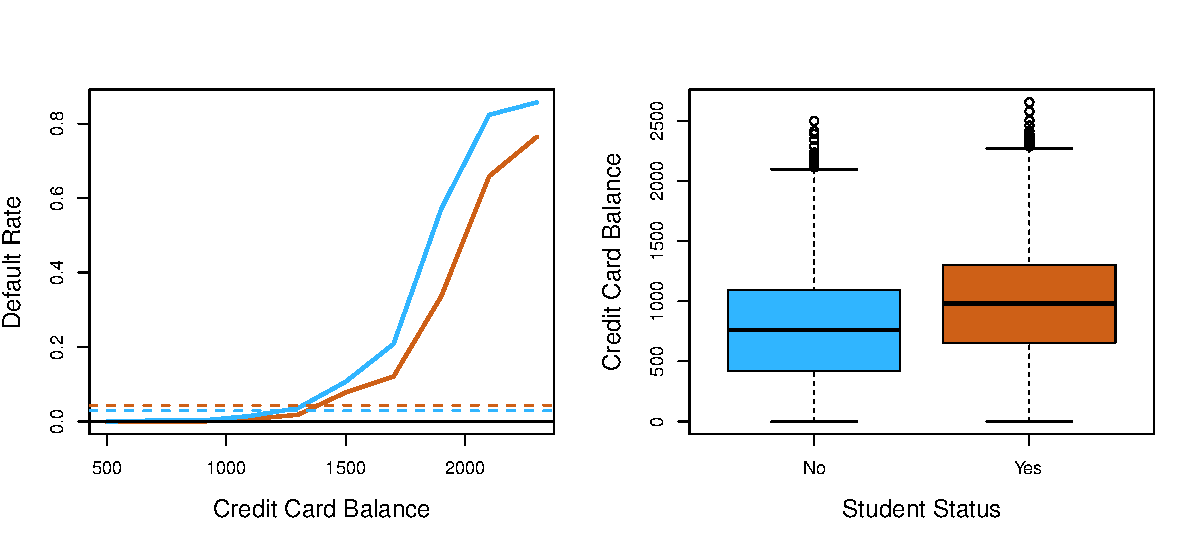
\includegraphics[width=.7\textwidth]{4-3}}

{\small A student is riskier than a non-student if no information about the student's credit card balance is available. However, that student is less risky than a non-student with the \emph{same credit card balance}.}

\end{frame}

\begin{frame}{Logistic regression}\large

\begin{itemize}
\item We define the \emph{odds} as $\frac{p(X)}{1 - p(X)}$ 
\item Example: $p(X) = 0.2$ and $p(X) = 0.9$
\item Odds close to $0$ and $\infty$ $\rightarrow$ very low and very high probabilities of default, respectively.
\item Log-odds (or logit) is linear in $X$: $log(\frac{p(X)}{1 - p(X)}) = \beta_0 + \beta_1 X$
\end{itemize}

\end{frame}




\begin{frame}{Evaluation of classifiers}\large


$\text{\alert{default} = \alert{Yes}} \text{~if~} \scriptsize \hat p(\text{\alert{balance}}) > 0.5 $
\centerline{
\includegraphics[width=.7\textwidth]{Table4}}

$\text{\alert{default} = \alert{Yes}} \text{~if~} \scriptsize \hat p(\text{\alert{balance}}) > 0.2 $
\centerline{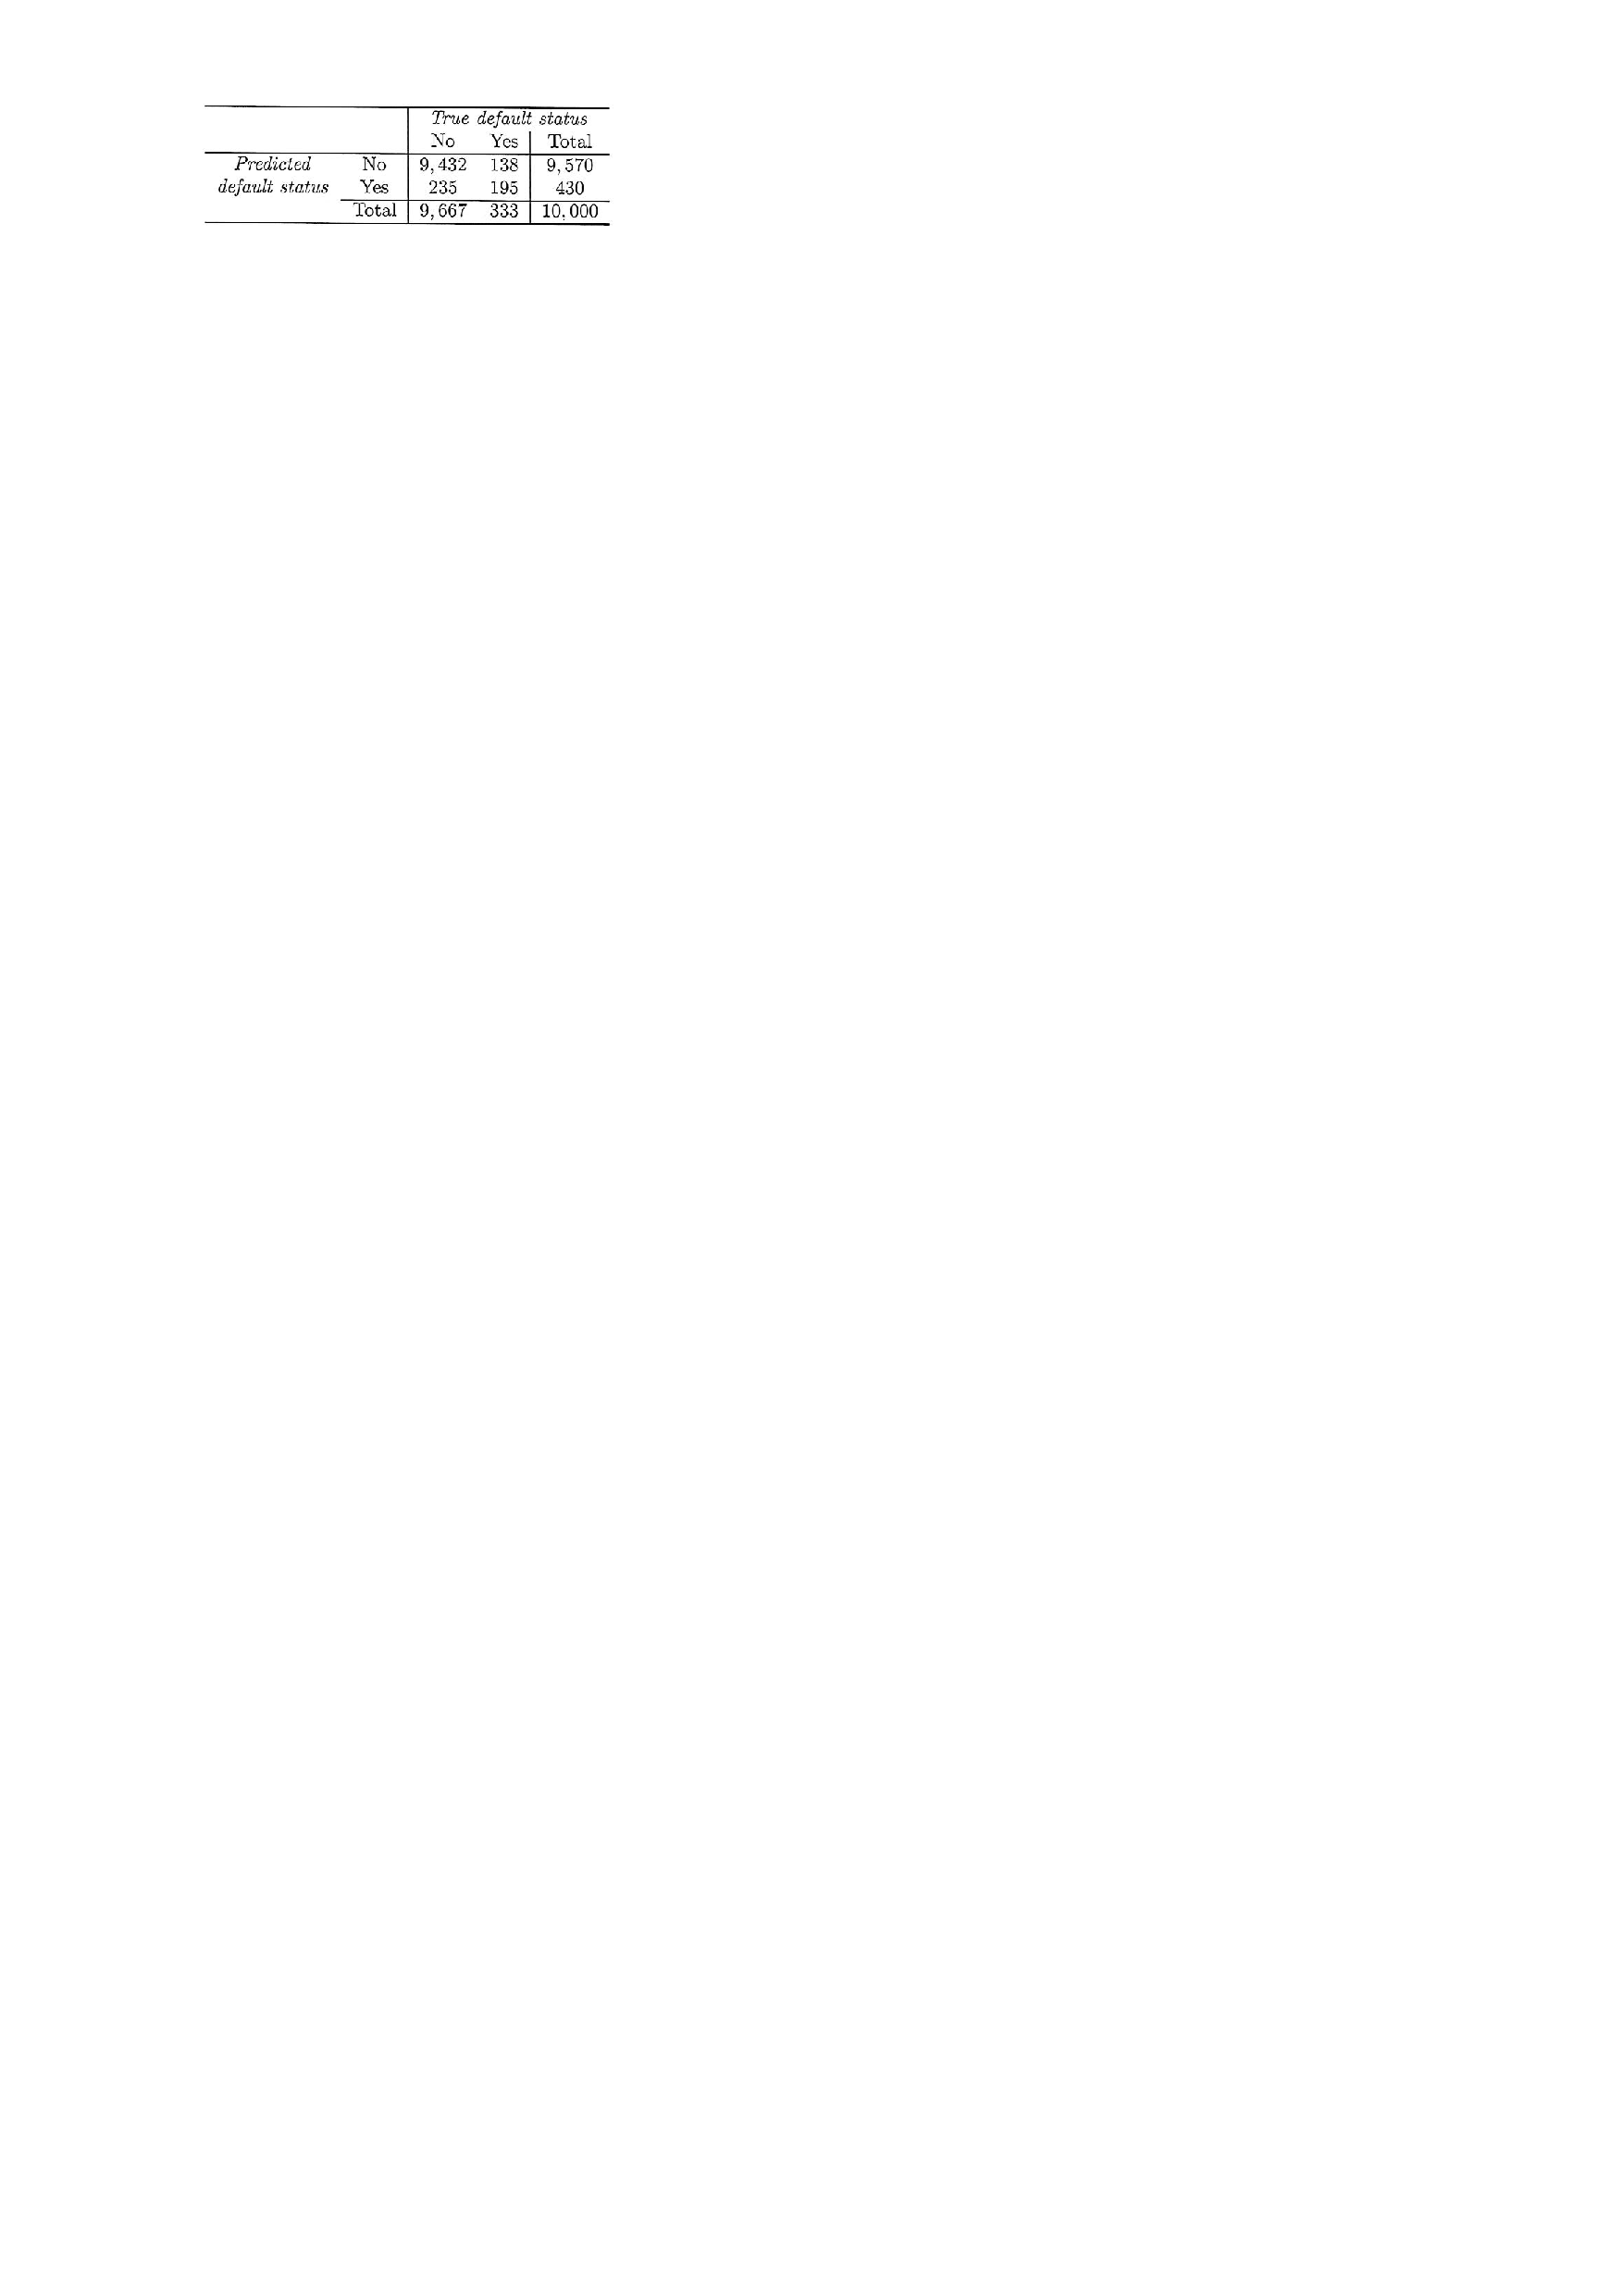
\includegraphics[width=.7\textwidth]{Table5}}



\end{frame}

\begin{frame}{Evaluation of classifiers}\large


\centerline{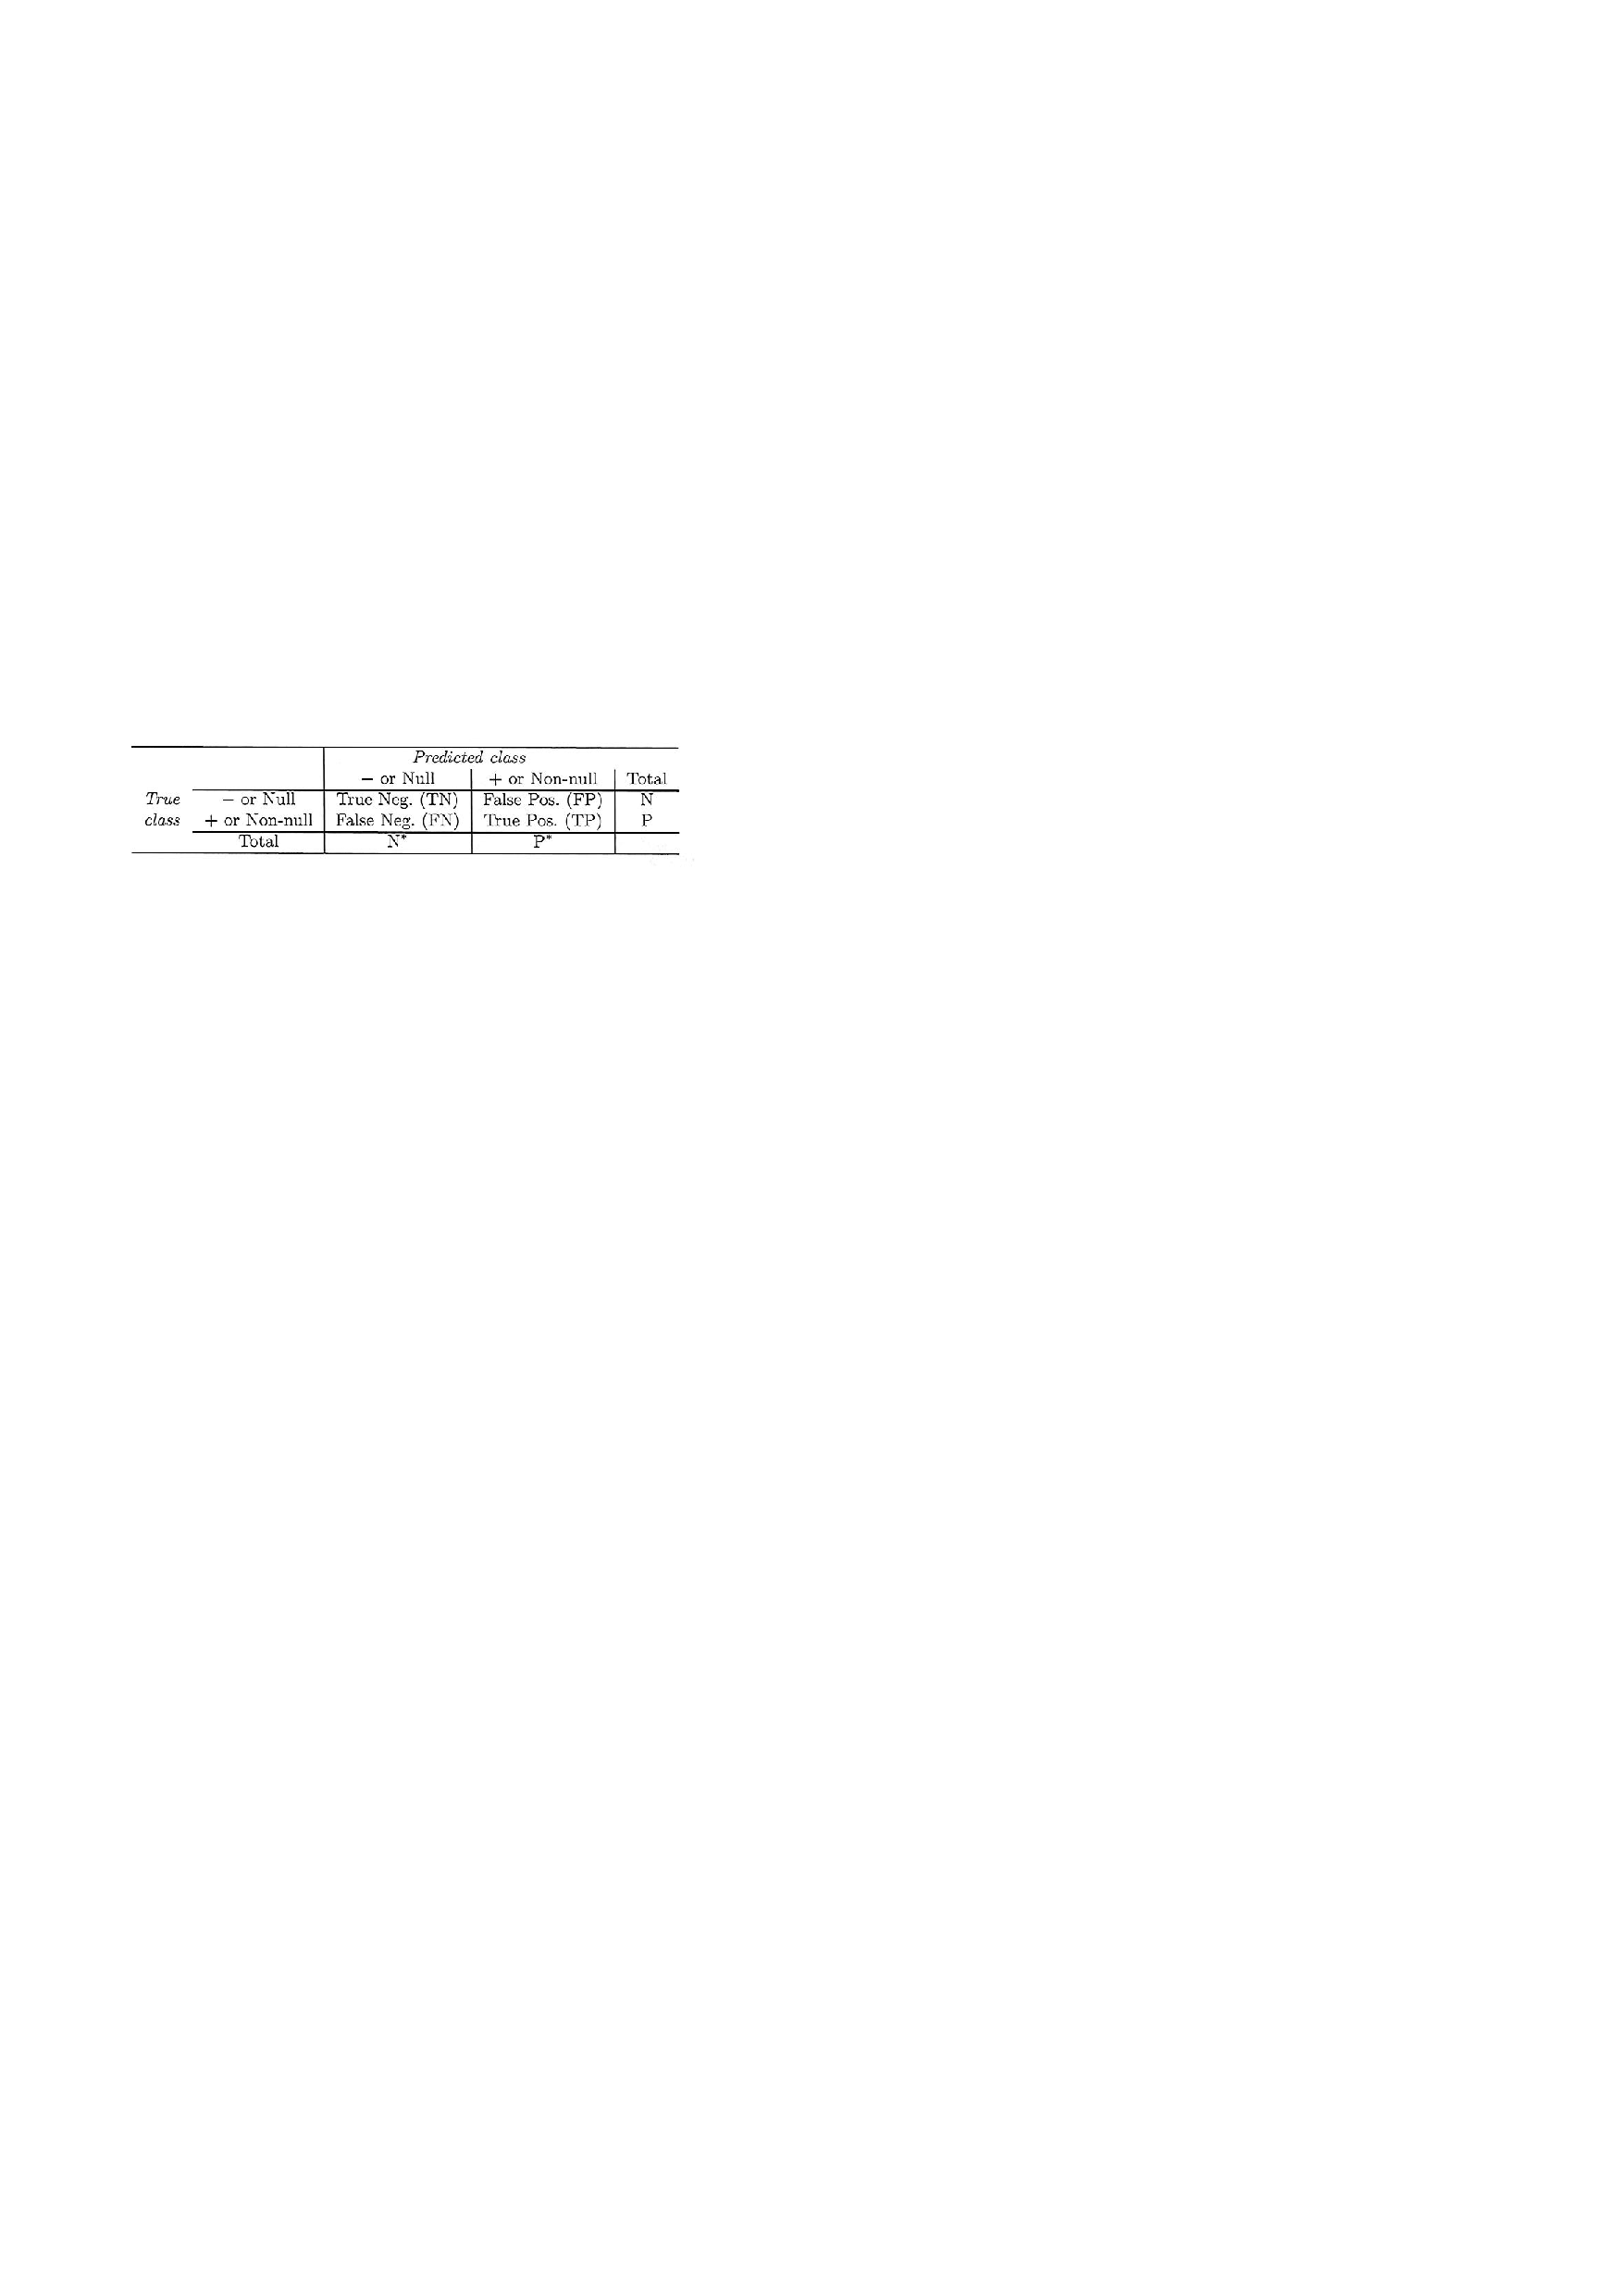
\includegraphics[width=.7\textwidth]{Table6}}

\centerline{
\includegraphics[width=.7\textwidth]{Table7}}


\end{frame}

\begin{frame}{Evaluation of classifiers}\large

\centerline{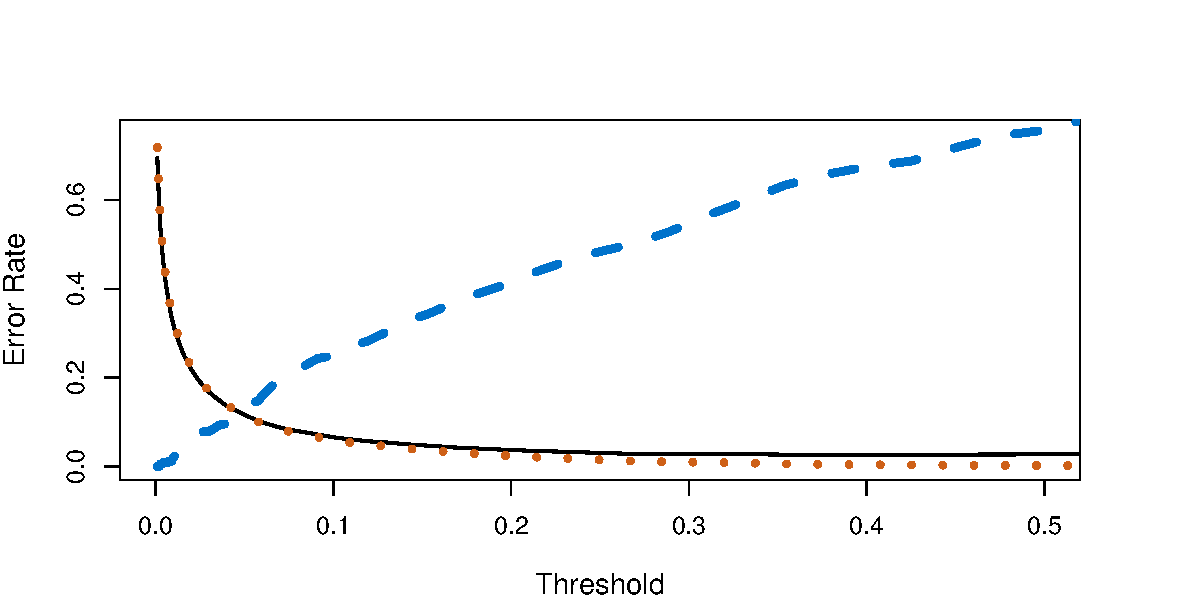
\includegraphics[width=.55\textwidth]{4-7} 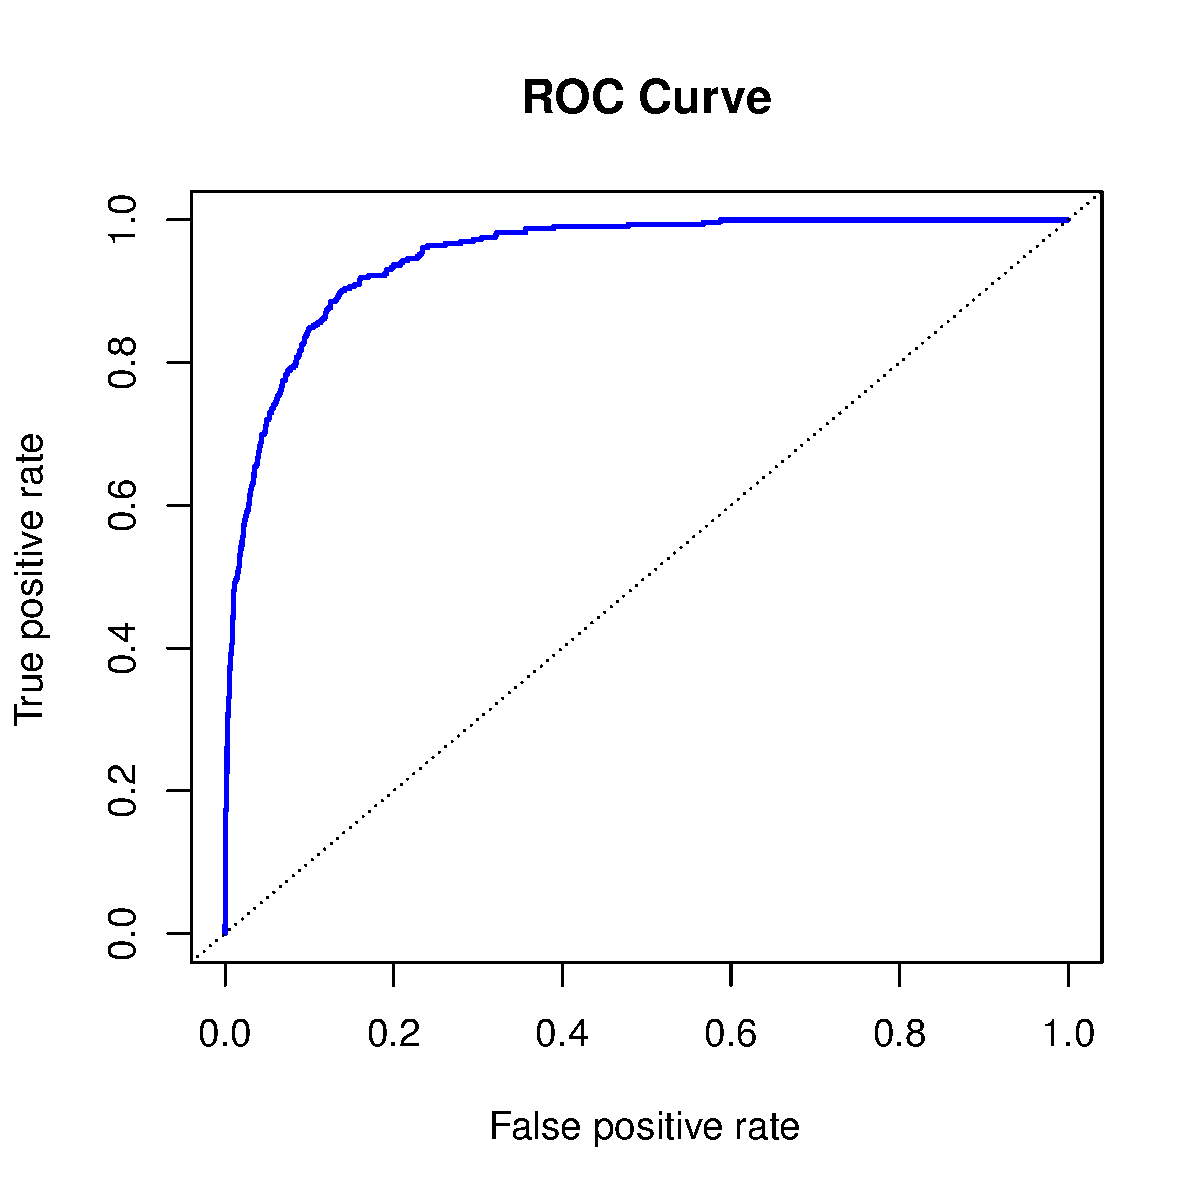
\includegraphics[width=.5\textwidth]{4-8}}

\end{frame}

%\begin{frame}{Multiclass classification}\large
%\end{frame}


\begin{frame}{Next class}

\begin{center} \textcolor{blue}{Linear Discriminant Analysis} \end{center}

\end{frame}



\end{document}